\section{Thiết kế quan niệm}

Thiết kế quan niệm mô tả dữ liệu ở mức nghiệp vụ, chưa phụ thuộc vào SQL Server hay một hệ quản trị cụ thể. Các danh từ trong yêu cầu được dùng làm ứng viên thực thể; các động từ và quy tắc nghiệp vụ được dùng để xác định mối kết hợp.

\section{Danh sách thực thể}

Các thực thể chính của OISM gồm:

\begin{table}[H]
\centering
\caption{Các thực thể và ý nghĩa nghiệp vụ}
\label{tab:concept-entities}
\small
\begin{tabular}{|p{0.36\textwidth}|p{0.51\textwidth}|}
\hline
\textbf{Thực thể} & \textbf{Ý nghĩa} \\
\hline
TENANT & Tổ chức sở hữu dữ liệu; dùng để cô lập dữ liệu. \\
\hline
ROLE & Vai trò/quyền truy cập. \\
\hline
USER & Người sử dụng hệ thống. \\
\hline
BRANCH & Cửa hàng hoặc kho thuộc tenant. \\
\hline
CATEGORY & Nhóm sản phẩm. \\
\hline
BRAND & Thương hiệu sản phẩm. \\
\hline
PRODUCT & Thông tin sản phẩm ở mức khái quát. \\
\hline
PRODUCT\_VARIANT & Biến thể có thể bán; trong mô hình logic được định danh bằng SKUId. \\
\hline
BARCODE & Mã dùng để nhận diện/tra cứu SKU. \\
\hline
PRICE & Lịch sử giá bán theo thời gian hiệu lực. \\
\hline
INVENTORY\_LEDGER & Lịch sử các biến động tồn kho, chỉ ghi thêm. \\
\hline
INVENTORY\_BALANCE & Số dư hiện tại phục vụ đọc nhanh. \\
\hline
PURCHASE\_RECEIPT & Phiếu nhập hàng. \\
\hline
PURCHASE\_RECEIPT\_ITEM & Chi tiết SKU trong phiếu nhập. \\
\hline
ORDER & Đơn hàng chuẩn hóa từ các kênh. \\
\hline
ORDER\_ITEM & Chi tiết SKU và số lượng bán. \\
\hline
RESERVATION & Lượng tồn đang được giữ cho đơn hàng. \\
\hline
STOCK\_TRANSFER & Phiếu chuyển hàng giữa hai chi nhánh. \\
\hline
STOCK\_TRANSFER\_ITEM & Chi tiết SKU trong phiếu chuyển. \\
\hline
STOCKTAKE & Phiếu kiểm kê. \\
\hline
STOCKTAKE\_ITEM & Chi tiết kiểm kê theo SKU. \\
\hline
\end{tabular}
\end{table}

\section{Mối kết hợp và bản số}

Các quan hệ chính:
\begin{itemize}
    \item TENANT $1:N$ USER, BRANCH, CATEGORY, BRAND, PRODUCT, SKU, ORDER;
    \item ROLE $1:N$ USER;
    \item CATEGORY $1:N$ PRODUCT; BRAND $1:N$ PRODUCT;
    \item PRODUCT $1:N$ PRODUCT\_VARIANT/SKU; SKU $1:N$ BARCODE và PRICE;
    \item BRANCH $1:N$ INVENTORY\_LEDGER và INVENTORY\_BALANCE;
    \item SKU $1:N$ INVENTORY\_LEDGER và INVENTORY\_BALANCE;
    \item PURCHASE\_RECEIPT $1:N$ PURCHASE\_RECEIPT\_ITEM; SKU $1:N$ PURCHASE\_RECEIPT\_ITEM;
    \item ORDER $1:N$ ORDER\_ITEM; SKU $1:N$ ORDER\_ITEM;
    \item ORDER $1:N$ RESERVATION; SKU $1:N$ RESERVATION;
    \item STOCK\_TRANSFER $1:N$ STOCK\_TRANSFER\_ITEM;
    \item STOCKTAKE $1:N$ STOCKTAKE\_ITEM.
\end{itemize}

Quan hệ nhiều-nhiều được chuyển thành thực thể liên kết. Ví dụ, ORDER và SKU có quan hệ nhiều-nhiều nên cần ORDER\_ITEM để lưu số lượng, giá bán và giá vốn của từng SKU trong đơn.

\section{Phân biệt thực thể và thuộc tính}

Một khái niệm nên trở thành thực thể khi nó có vòng đời riêng, có nhiều thể hiện, có thuộc tính cần lưu và thường xuyên được tra cứu/cập nhật. Ví dụ, ``SKU'' là thực thể vì được tham chiếu bởi tồn kho và đơn hàng; ngược lại, ``ProductName'' là thuộc tính mô tả PRODUCT.

\section{ERD}

Hình ERD phải thể hiện tên thực thể, khóa định danh, các quan hệ và bản số. Đây là đầu ra trung tâm của thiết kế quan niệm.

\begin{figure}[H]
    \centering
    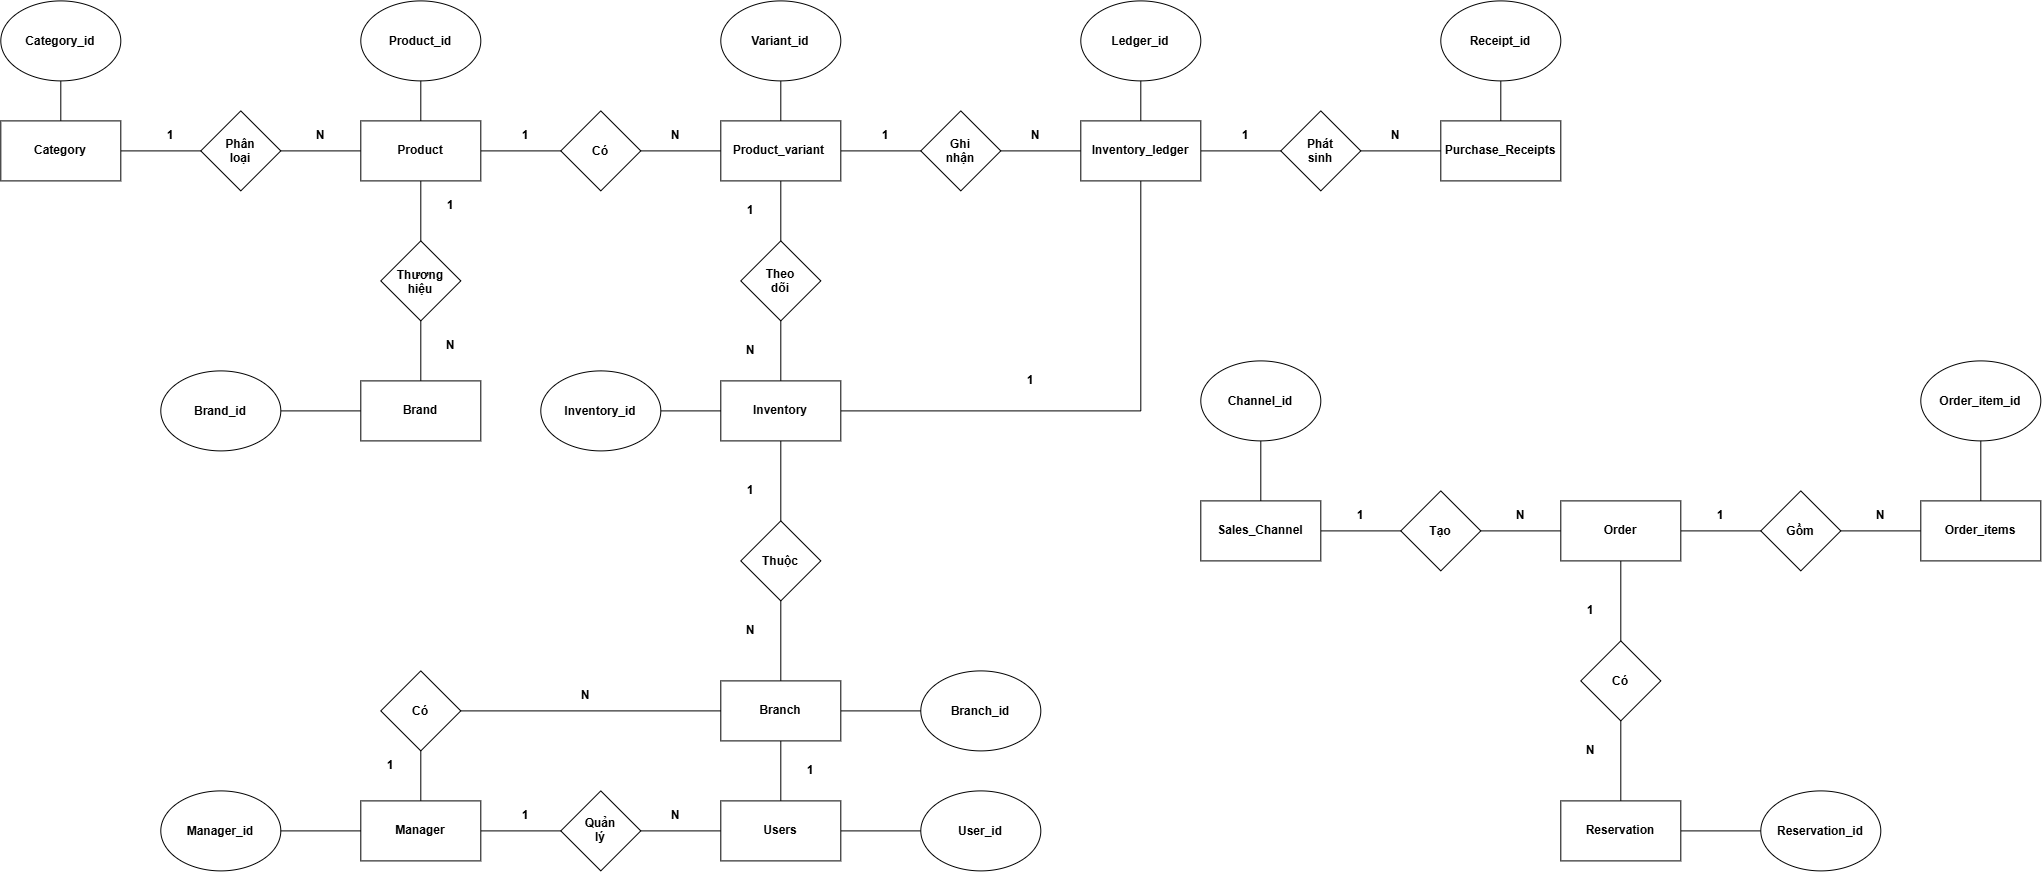
\includegraphics[width=0.92\textwidth,keepaspectratio]{figures/ERD.png}
    \caption{ERD của hệ thống OISM}
    \label{fig:erd-database}
\end{figure}
